\documentclass{sig-alternate}

\begin{document}
	\title{CSCI-620 Data Mining with the Airbnb Dataset}
	\subtitle{[Exploring and Mining the dataset of NY Airbnbs]}
	
	\numberofauthors{4}
	\author
	{
		\alignauthor
		Aishwarya Rao
		\email{ar2711@rit.edu}
		\alignauthor
		Apurav Khare
		\email{ak2816@rit.edu}
		\and
		\alignauthor
		Martin Qian
		\email{jq3513@rit.edu}
		\alignauthor
		Prateek Kalasannavar
		\email{pk6685@rit.edu}
	}
	
	\maketitle
	\begin{abstract}
		
		Data mining and its scope has grown tremendously over the last decade and is now an integral part of our lives. This project aims to perform a data mining task to explore the field as well as understand identify the scope of prediction in the selected dataset. The phases are planned accordingly to improve the measure with each step. 
		
	\end{abstract}
	
	\section{introduction}
	
	\subsection{The New York City Airbnb Dataset}
	The New York City Airbnb dataset is a dataset available on Kaggle which consists of data of hosts, locations and prices for Airbnb in New York in 2019. The dataset consists of attributes such as name, location in latitude and longitude, neighborhood, room type and price. The dataset consists of around 5000 rows. 
	
	\subsection{Choosing the dataset}
	There are a multitude of reasons why this dataset was appealing. They are as follows,
	\begin{itemize}
		\item The dataset is based on real data which makes the data mining task more practical - both in terms of use case scenarios as well as complexity of the data.
		\item With around 5000 rows, the dataset size is optimal for a data mining task. It is not too large to create needless challenges but not too small to prevent generalization.
		\item The dataset is open source and is updated annually. 
	\end{itemize}
	
	\subsection{The Data Mining Task}
	\subsubsection{Prediction}
	One important usage of data mining is to perform predictions, especially for commercial
	datasets. For our dataset, we choose to use a data mining algorithm to predict the price range for a new Airbnb host in New York City. That would allow new hosts to estimate the price for their listings for maximum interaction. 
	\subsubsection{Evaluation}
	With this idea of predicting the price category in mind, we explored the dataset to confirm with our assumption that this task is actually possible through the data present. As seen in the figure, the price column is distributed reasonably well. It is possible to map these into bins for further predictions. Furthermore, through exploration of the dataset, we found correlation between price and multiple other attributes in the dataset. With this information, we decided to go forth with predicting the price in the dataset. 
	\begin{figure}[ht]
		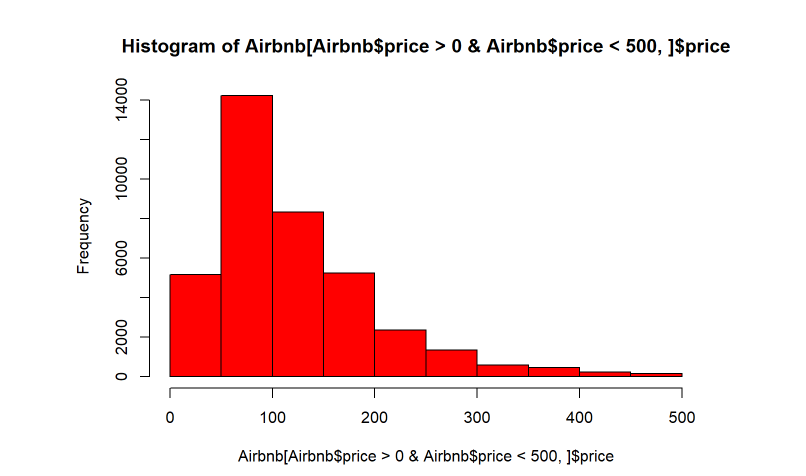
\includegraphics[width=9cm]{hist.png}
		\label{hist}
		\centering
	\end{figure} 
	\subsubsection{Integration}
	We all know that apart from the data itself, there are many other outside factors that can 
	have impact on the data. Outside of the information in the dataset, we are considering integrating the data with some other factors like the map information of the New York City, safety level of the neighborhood and so on.
	This task will involve finding datasets that can be with our current dataset. Through this integration, we hope to be able to present our findings from the prediction in a more user-friendly and understandable manner. 
	
	\subsection{Proposed method}
	Several different data mining algorithms exists for classification including decision trees, SVM and K-Means. We plan to perform classification and evaluation on the price by splitting it into bins. 
	Evaluation will be measured by accuracy. The project will be coded in R. 
	
	\section{Future plan}
	Week 9: Preparation and dataset selection
	
	Week 10-11: Data features analysis, feature engineering, shortlist classification algorithms
	
	Week 12-13: Run algorithm and make improvements based on precision and accuracy.
	
	Week 13-14: Visualizations, inferences based on our final model.
	
\end{document}